\chapter{Introduction}
\label{chap:introduction}

\begin{figure}[h]
    \centering
    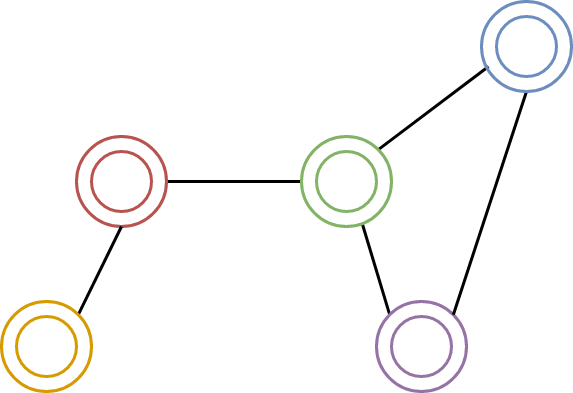
\includegraphics[scale=0.2]{graphics/mesh.png}
\end{figure}

Consider an application that is distributed over a network, e.g. as a set of \textit{Internet of Things}-devices (IoT). The
connection between devices forms a mesh network, and for the devices to be able to cooperate and implement the application they
need to agree on facts such as what the current time is, what other devices are part of the network, and more. In many cases
IoT devices take one of two roles. Either a device will perform period tasks such as reading a sensor and then transmitting
the value across the network to other devices, or a device will be idle until a value arrives from another device, at which point
the device needs to \textit{react} to that value.

The application described above has many moving parts that are non-trivial. The scarcity of hardware resources on many IoT
devices means that devices are often forced to rely on a battery for power. To ensure the continued availability of devices,
they need to carefully manage their power consumption such that the battery life is extended as far as possible. In addition to 
this, temporal properties need to be carefully stated and implemented. It could be crucial that future action is
performed at a very precise moment in time. For devices to form a mesh network
and cooperate, the devices need to manage cryptographic keys. These keys are used to decide if a device is part of the network
or not and to ensure that a message in transit from one device to another is encrypted, such that the integrity of the network
is not violated.

The above requirements are very pervasive during the development of such an application and must be considered at every stage of
development. Devices such as these are usually programmed using low-level languages and toolchains such as C/C++. All the
requirements of the application above will require a lot of boilerplate code. Many things need to
happen to ensure that the requirements are met but don't relate to the application logic. Furthermore, the lack of features
such as memory safety makes code error-prone.

High-level languages offer different language abstractions that can more easily express the desired behavior of an application.
In addition, a language could offer domain-specific abstractions that ease application development for a specific domain.
As an example, aside from being a general-purpose language, Haskell's support for custom algebraic datatypes and pattern-matching
make Haskell excel at implementing programs that need to manipulate trees, such as compilers and interpreters. Erlang's support
for spawning concurrent processes that can communicate between endpoints in a network makes Erlang a good choice for implementing
applications that need to be distributed and scalable.

We ask ourselves a question; can we leverage high-level languages with domain-specific abstractions to ease the
development of applications such as the one described at the top of this section? If the developer can be freed from the burden
of having to maintain boilerplate code, the developer can focus on what the application is supposed to do, rather than
details of how it does it.

The topic of this thesis is to investigate whether it is feasible to develop a high-level language that meets the requirements
of the application domain described above.
requirements. To
answer this, we develop DSLs that explore what domain-specific abstractions may be useful. The languages are
implemented as \textit{embedded} domain-specific languages (DSL) in the functional language Haskell. Embedding a DSL in a host
language drastically reduces the initial cost of language development, and enables experimentation to commence much quicker. An
embedded language can be implemented as an embedded compiler that generates code to be executed later, or as an embedded
interpreter that runs the program during host language execution time.

While we don't yet have a full story and a definitive answer, the work in this thesis brings us closer.
The thesis presents two DSLs, Scoria and HasTEE. Scoria investigates domain-specific
abstractions that help a developer specify the temporal behavior of their program. Additionally, the runtime system of Scoria can
recognize that a long period of inactivity is coming, and can choose to put the device it is running on in a low-power mode,
to conserve energy. While we have not evaluated how much power can be conserved yet, we believe it will be easy to evaluate
in the future. Scoria is intended to run on microcontrollers with scarce resources. Given the extensive runtime demands
of Haskell, it becomes infeasible to employ Haskell as the execution vehicle. Consequently, to address this limitation, Scoria
is implemented as an embedded compiler that generates C code. The C code is compiled at a later stage and executed on the device.

HasTEE develops domain-specific abstractions that ease the development of software with security requirements. Specifically,
HasTEE enables a developer to use the type system of Haskell to identify the parts of an application that are to be executed in a
trusted execution environment (TEE). The type system encodes a variant of information-flow control (IFC), but where traditional
IFC threat models require a developer to trust an underlying operating system, HasTEE does not require trust in an operating system.
A HasTEE application is automatically partitioned into two programs, an untrusted program and a trusted program, with the trusted
program being executed in a hardware-enforced TEE. The developer does not need to care about how confidentiality
is achieved when developing the application. HasTEE is intended to run on machines with more resources than that of the target
platform of Scoria, and as such is implemented as an embedded interpreter, where HasTEE uses the Haskell runtime as its execution
vehicle.

The results of this thesis indicate that there is space for a high-level language with domain-specific abstractions
that will ease application development in this domain, and many interesting lines of future work could be pursued.
First, we wish to draw some synergy between Scoria and HasTEE and enable a developer to write Scoria programs that use TEEs on
microcontrollers, e.g. Arm TrustZone on Cortex-M processors. Second, we wish to investigate if we can extend Scoria with
functionality to describe complete networks of devices and generate code for each of them. We wish to use the type system of
Haskell to identify unique devices and partition an application based on that.

In the remaining part of this introduction, we start by introducing the two domains that the DSLs presented in this thesis
focus on. We describe these domains using an example application and discuss specific aspects of application development
within each domain. Additionally, we explore domain-specific features that can facilitate development. Following that, a 
background section covers core topics that are pertinent to this thesis. Finally, the two papers will be presented.

% \begin{itemize}
%     \item The network is the computer - John Gage
%     \item Start from a high view, describing a distributed application with temporal behavior and
%     confidentiality requirements. From there, zone in on the difficulties with developing
%     these applications. (Low-level languages, power requirements, timing requirements, confidentiality requirements)
%     The impact is very pervasive
%     \item Low-level toolchains lead to a lot of code, which is more likely to be erroneous. Huge amount of
%     boilerplace code obfuscates application logic. Wish to use a high-level language to describe what the
%     application should do, without necessarily specifying how.
%     \item My plan - a high-level language for this
%     \item Embedded language development, quick prototyping, reuse components, high-level! Embedded compiler vs embedded interpreter.
%     \item Selling-point of HasTEE - partitioning and non-obfuscated application logic in the confidential component
%     \item Selling-point of Scoria - Time is native, sparse model, good for power requirements, High-level
%     \item Remaining work: Distributed Scoria, tierless programming, Arm TrustZone for confidential Scoria
% \end{itemize}

\section{Programs with Temporal Behaviors}

Consider a simple program
that flashes an LED at a fixed frequency. This program is the "Hello world!" of microcontroller programming and is often distributed
as an example application with operating systems for microcontrollers. It illustrates how to perform
periodic tasks that do IO. The desired output should vary over time as illustrated in figure \ref{graphics:correct-frequency}.

\begin{figure}
    \centering
    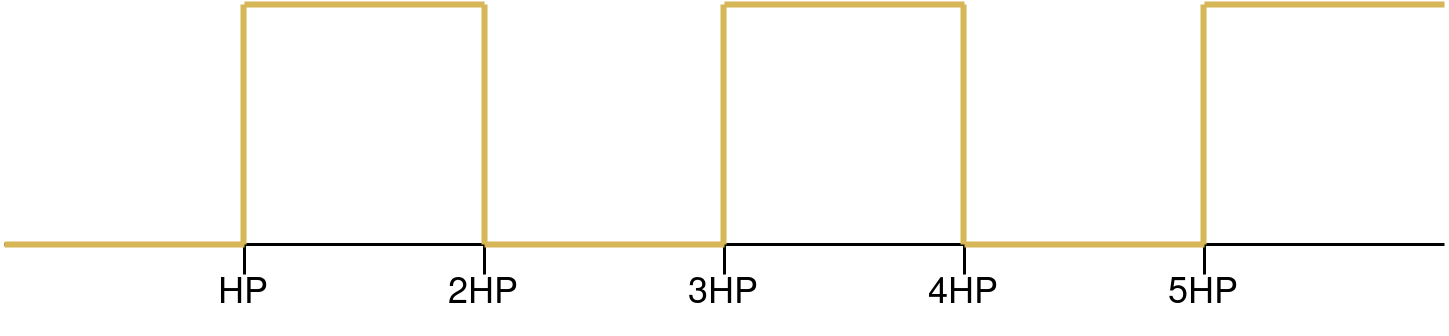
\includegraphics[scale=0.2]{graphics/correct-frequency.png}
    \caption{The yellow line denotes the LED state and its desired temporal behavior. The desired behavior
    is that it is turned on and off with a stable frequency, with each change in state occurring at the
    half-period points, denoted \code{HP} in the diagram.}
    \label{graphics:correct-frequency}
\end{figure}

A pseudo-code variant of the program, as it is often illustrated, is shown below.

\begin{verbatim}
    void main() {
        while(1) {
            toggle_led(the_led);
            sleep(half_period);
        }
    }
\end{verbatim}

An equivalent version of the same program could use alarms and callbacks to specify what should happen at what time. Such
a version of the program appears below.
\begin{verbatim}
    void toggle() {
        toggle_led(the_led);
        set_alarm(half_period, &toggle);
    }

    void main() {
        configure_timer();
        set_alarm(half_period, &toggle);
    }
\end{verbatim}

The main function above configures some timer and sets an alarm that, when the alarm goes off, will trigger an invocation of
the \code{toggle} function. The \code{toggle} function flips the current value of the LED and then sets a new alarm.
While the code is very simple and seems to implement the desired semantics, it is buggy! The frequency will not be
the one we want. When the alarm goes off and the function is invoked, the function performs some operations before the next
alarm is set. If we call the time it takes to perform the operations $\delta_{op}$ and the half period $hp$, the times the
alarm goes off are $$0, \delta_{op} + hp, 2(\delta_{op} + hp), 3(\delta_{op} + hp), 4(\delta_{op} + hp), ...$$

This sequence illustrates that, as time progresses, the frequency drifts further and further away from the target. See
figure \ref{graphics:drift}.

\begin{figure}
    \centering
    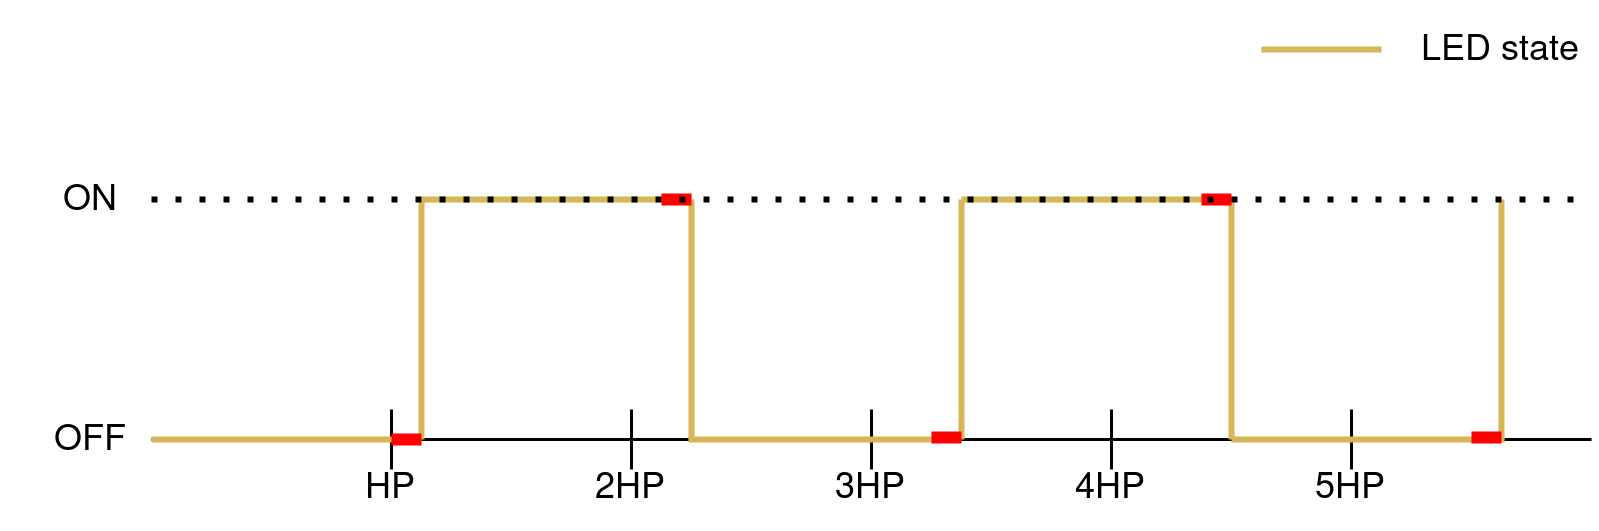
\includegraphics[scale=0.2]{graphics/drift.png}
    \caption{The diagram illustrates where the half-period points are, and where the change in LED state occurs.
    The red segments illustrate the time $\delta_{op}$. The additions of $\delta_{op}$ lead to the frequency of the change in
    LED state drifting further and further away from the half-period points.}
    \label{graphics:drift}
\end{figure}

Let us try to fix our program to allow for the time it takes to perform the operations.
As soon as \code{toggle} is invoked, we query the system for the current time. The next time we set
the alarm we configure the alarm to go off relative to the previously sampled time.

\begin{verbatim}
    time current;

    void toggle() {
        current = current_time();
        toggle_led(the_led);
        set_alarm_relative_to(current, half_period, &toggle);
    }

    void main() {
        configure_timer();
        current = current_time();
        set_alarm_relative_to(current, half_period, &toggle);
    }
\end{verbatim}

Even with the alarm set relative to when the process last woke up, the frequency suffers from drift. An oscilloscope
will report that the drift is smaller than before, but still present. This remaining source of drift is a bit
trickier to account for.

When the actual hardware clock reaches the point where an alarm should be raised, it takes some time for the
operating system to locate the \code{toggle} function and invoke it. To account for this delay, we can choose to
set alarms not relative to when \code{toggle} was last invoked, but rather relative to when \code{toggle}
\textit{was supposed} to have been invoked. We do this by implementing a logical clock that is incremented to reflect
what the time of the system should be.

\begin{verbatim}
    time current;

    void toggle() {
        current = current + half_period;
        toggle_led(the_led);
        set_alarm_absolute(current + half_period, &toggle);
    }

    void main() {
        configure_timer();
        current = 0;
        set_alarm_absolute(current + half_period, &toggle);
    }
\end{verbatim}

The program now maintains a global variable that tracks the current time. An absolute alarm is set that will go off at
time \code{current + half\_period}, regardless of what time it is when the alarm is set. The next time \code{toggle}
is invoked, it is assumed that time has progressed to \code{current + half\_period}, and the logical time is updated
to reflect this. If the system time is queried at this point, it will show that the current time is 
\code{current + half\_period +} $\delta_{lookup}$, where $\delta_{lookup}$ is the amount of time it takes for the
\code{toggle} function to be found and invoked.

Executing this program will flash the LED with the correct frequency. Since the delay for the system to look up and
invoke the callback ($\delta_{lookup}$) is still there, there is a small phase error (the size of which is equal to
$\delta_{lookup}$), but the frequency is still stable and correct. The LED state is illustrated in figure \ref{graphics:phase-error}

\begin{figure}
    \centering
    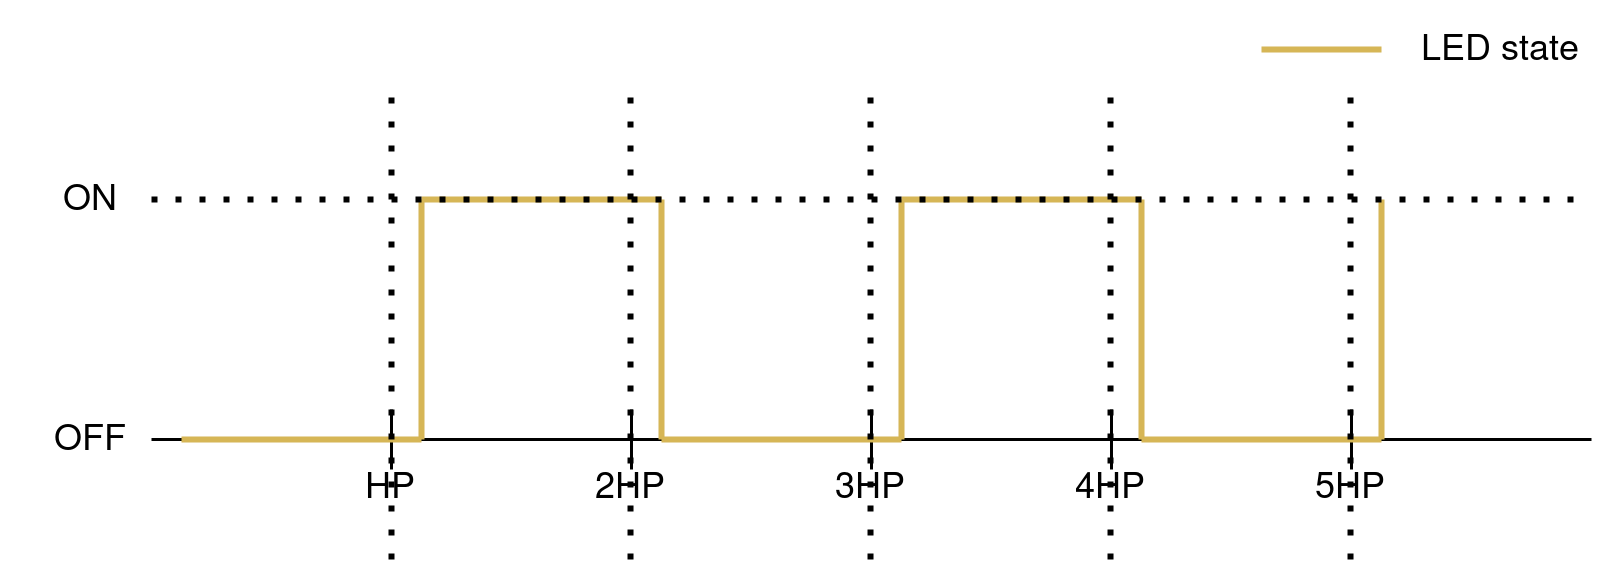
\includegraphics[scale=0.2]{graphics/phase-error.png}
    \caption{The diagram illustrates the frequency of the change in LED state in the final version of the program.
    There is a small phase error, indicated by the dotted lines, but otherwise, the frequency is the expected one.
    The dotted lines denote the actual half-period points, and the distance from the points where the LED state
    changes to the half-period points remain constant. The distance is of duration $\delta_{lookup}$.}
    \label{graphics:phase-error}
\end{figure}

While the initial program seemed intuitively reasonable, it was erroneous. The final version is
correct (up to the phase error), but is substantially more complicated. While the pseudo-code might look short and
simple, still, we now have a program that maintains a logical time and sets absolute deadlines, something that is easy
to get wrong.

The extra complication is a result of the primitive timing API in a language such as this. Querying the system for the current
time and setting alarms is a very coarse API. The fact that the system does not assist the developer with accounting for
systematic delays and the time it takes to perform computations makes the whole business of reasoning about deadlines much more difficult.

Domain-specific abstractions that would make writing this program simpler are
\begin{itemize}
    \item An abstraction that schedules an alarm to go off after a certain amount of time
%    \item specify very precise periods of rest (where a software 'pauses') -- we can synthesize this
    \item An abstraction that yields control while awaiting an alarm
\end{itemize}

A developer should be able to use these primitives without thinking about systematic delays like the ones discussed above.
The logical time should be maintained by the runtime system. A rewrite of the above program using functionality of this
kind yields

\begin{verbatim}
    void main() {
        alarm a = new_alarm();
        while(1) {
            toggle_led(the_led);
            set_ds_alarm(half_period, shared);
            wait(shared);
        }
    }
\end{verbatim}

The program looks very similar to the first version, except for using an explicit alarm instead of an
invocation of a \code{sleep} function.

The first paper in this thesis describes work in this domain. A domain-specific language, which we call
Scoria \cite{DBLP:conf/memocode/KrookHSEC22}, is implemented as an \textit{embedded} language in Haskell. While Scoria
has primitives similar to the ones described above, the alarms are more expressive. Alarms take the form of mutable
variables, which always have a value. An update to a mutable variable can be scheduled for the future, while a process can
choose to block until a mutable variable receives an update. The conceptual alarm goes off when the update occurs, and with
this alarm comes a value (the new value of the variable).

\begin{verbatim}
    signal_generator :: Ref Output -> Time -> SSM ()
    signal_generator led hp = routine $ while True $ do
        after hp led (invert $ deref led)
        wait led
\end{verbatim}

In this program, the LED variable itself becomes the alarm. In a while loop, a future update is scheduled for the LED
variable after which the program blocks until the update occurs. In Scoria, by writing to a variable associated
with an LED, the value of the LED is immediately propagated to the physical LED.

\section{Programs with Confidentiality requirements}

The second application domain investigated in this thesis is that of confidential computing. Confidential computing is
the act of protecting \textit{data in use}.
Data always exists in one of three states. It can exist as \textit{data in motion}, as \textit{data at rest}, or as
\textit{data in use}. Data in motion is data that is moving from one part of the system to another, e.g. via TCP, while data at rest
is data that is being stored in persistent memory. Both of these kinds of data can be protected via e.g. encryption.
Encryption is enough to guarantee confidentiality in these cases if you trust your encryption scheme.

Data in use, however, is a bit different. To perform any meaningful operations on data, it has to be loaded into the RAM.
Consider the pseudo-code below, that stores secrets persistently in an encrypted data store. For illustrative purposes, the
data store variable is used as if it represents the data directly, but can also represent a file handle or something more
realistic.

\begin{verbatim}
    ciphertext encrypted_data_store;

    bool process_data(request req) {
        // decrypt data store
        plaintext decrypted = decrypt(encrypted_data_store);

        // compute result of request
        bool result = handle_request(decrypted, req);

        // update the data store
        plaintext new_data_store =
            update_data_store(result, decrypted);

        // encrypt and save data store
        encrypted_data_store = encrypt(new_data_store);
        return result;
    }

    void main() {
        while(true) {
            request req = await_request();
            bool result = process_data(req);
            print(result);
        }
    }
\end{verbatim}

The code above consists of two parts. The first part is the \code{main} function, that waits for and parses incoming
requests. The second part is the application logic. Here we decrypt the secret data, compute some result with it,
update it, and then encrypt it before we store it again.

A problem with this code is that the secret data is decrypted before it is operated on. The result of this is that it exists
in plaintext in the RAM of the machine the code is running on, and an attacker running on the same machine, such as a
compromised operating system, might leak this data. This is illustrated in figure \ref{graphics:unsafe-data-in-use}.

\begin{figure}
    \centering
    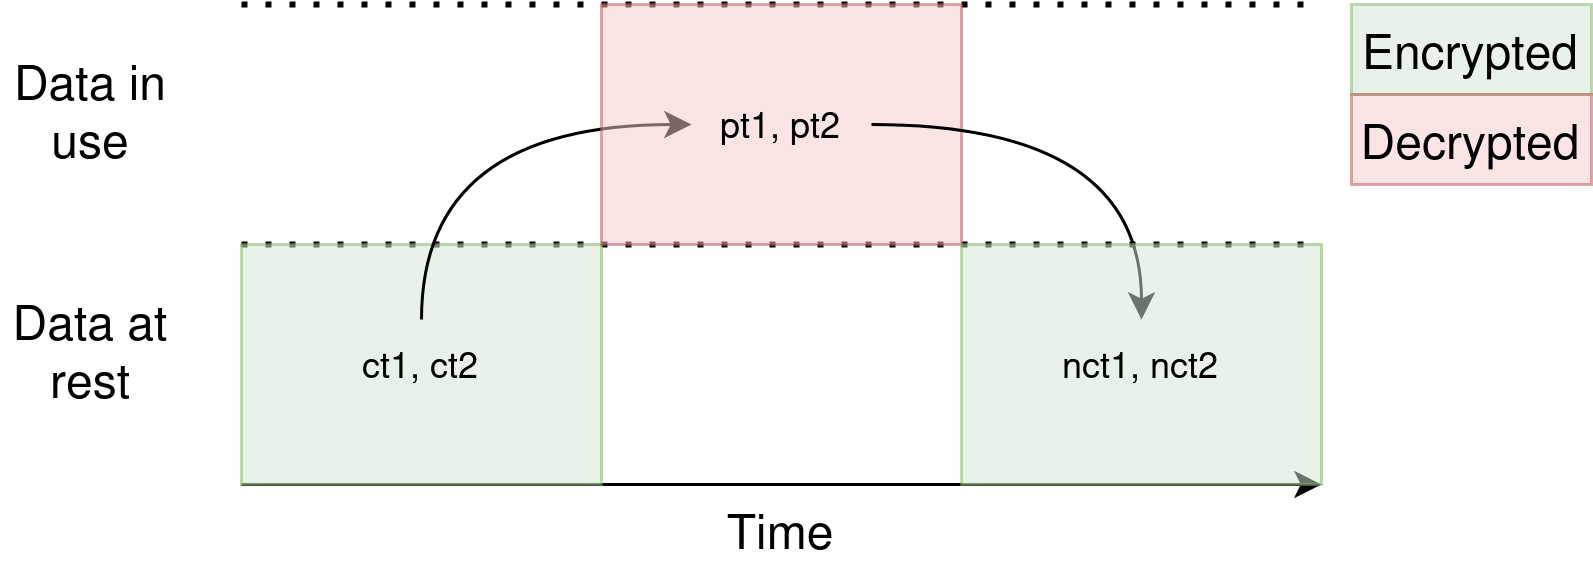
\includegraphics[scale=0.2]{graphics/unsafe-data-in-use.png}
    \caption{The diagram illustrates that while the data is at rest, it exists in encrypted form. When the data
    is operated on it is decrypted (as indicated by the red color), before the updated data is encrypted and stored.}
    \label{graphics:unsafe-data-in-use}
\end{figure}

To mitigate this vulnerability, we wish to modify the program such that the secret data does not have to reside in RAM in
a decrypted format. One approach to achieve this is to apply \textit{fully homomorphic encryption}
\cite{DBLP:conf/stoc/Gentry09} (FHE), which encrypts the data such that it can be operated on directly. Drawbacks with this
approach are that fully homomorphic operations on encrypted data are very slow and that there can be a substantial amount of
noise added to encrypted values. It takes an expert to write code that uses FHE such that it is feasible to execute it, both in
terms of execution speed and accuracy of the result. Furthermore, there is a risk that the application logic becomes obfuscated
if the code is using FHE.

Another mitigation technique, which we investigate in this thesis, is using TEEs to do confidential computing. The domain-specific
abstractions we investigate in this thesis are

\begin{itemize}
    \item Using the type system to identify which components of an application should reside in a TEE. If the return type of a
    procedure, or the type of a variable, is secure, that entity is expected to reside in a TEE.
    \item Allowing the result of a secure computation to be accessed outside of the TEE.
\end{itemize}

The above example, rewritten using these domain-specific abstractions, becomes

\begin{verbatim}
    secret plaintext data_store;

    secret bool process_data(request req) {
        // compute result of request
        secret bool result = handle_request(data_store, req);

        // update the data store
        secret plaintext new_data_store =
            update_data_store(result, data_store);

        // save data store
        data_store = new_data_store;
        return result;
    }

    void main() {
        while(true) {
            request req = await_request();
            bool result = inTEE(process_data(req));
            print(result);
        }
    }
\end{verbatim}

The type of the data store is now \code{secure plaintext}, denoting that it resides in the TEE and that there is no need to
protect the data further by encrypting it. Similarly, the procedure \code{process\_data} now returns a \code{secret bool}, indicating
that the procedure exists in the TEE. Procedures in the TEE are allowed to inspect \code{secret} variables, whereas if a procedure
outside of the TEE tries to inspect \code{secret} data, an exception is raised.
The \code{main} procedure, which resides outside of the TEE, invokes a procedure in the TEE by means of the \code{inTEE} method,
which invokes a secret procedure and extracts its result.

The point of using a TEE is to put as little code as possible in it. If the code inside the TEE is compromised, the entire TEE is
likely compromised. To this end, the (usually) very large operating system resides outside of the enclave. By using the type
system to encode what is confidential or not, the non-trivial task of partitioning a program can be done automatically by the
compiler, yielding a smaller executable for the TEE.

The second paper in this thesis presents the DSL HasTEE, which uses the type system of Haskell to discover which part of
an application should execute in a TEE, and which part should reside outside. An application is partitioned automatically,
and communication between the two components is inserted. The above program can be written in HasTEE, as shown below

\begin{verbatim}
processData :: Enclave (Ref DataStore) -> Request -> Enclave Bool
processData erd req = do
  ref       <- erd
  dataStore <- readRef ref
  let result = handleRequest dataStore req
  writeRef ref (updateDataStore result dataStore)
  return result

main :: App Done
main = do
  ref      <- liftSecureRef InitialEmptyDataStore
  procData <- secure $ processData ref
  runClient $ do
    sequence $ repeat $ do
      req    <- await
      result <- onEnclave $ procData <.> req
      putStrLn $ show result
\end{verbatim}

A Haskell developer will be very productive, very quickly, using HasTEE. The only HasTEE-specific language abstractions are
two monads, called \code{Enclave} and \code{Client}, which denote what must go into the TEE and what may not. The above
program will be partitioned into two components where \code{processData} will end up in the TEE, and \code{main} will
remain outside.

\section{Background}

This section describes core topics that are relevant to this thesis. The first topic is \textit{Embedded Domain-specific Languages},
as the research presented in this thesis has been carried out by implementing embedded DSLs.
After this, a section about \textit{Synchronous Programming Languages} follow, as the DSL presented in paper one, Scoria, belongs
to the class of synchronous languages.
The last two topics relate to the DSL presented in paper two, HasTEE. They are \textit{Information-flow Control} and
\textit{Trusted Execution Environments}.

\paragraph{Embedded Domain-specific Languages}

Implementing a programming language requires considerable engineering effort. At the very least, a parser and interpreter
has to be implemented. More than often there are many more phases involved, such as type checking, renaming, etc.

A lot of engineering effort can be spared by implementing a language as an embedded language. An embedded language is
implemented in another language, called the host language, as a library. By embedding a language in
a host language, many phases from the host compiler can be directly inherited by the new language, such as the parser,
type checker, code generator, etc.

Languages can be embedded in either a \textit{shallow} or \textit{deep} fashion.
When using a shallow embedding, an embedded program is executed during host language execution time. For better or worse,
this means that the embedded language inherits the host language's runtime. A deep embedding, in contrast, will
produce syntax during the language execution time, which can later be compiled and run independently of the host language.
In such a scenario we have two distinct execution times, the host language execution time, and the execution time of the generated
code, the embedded language. The host language becomes a very powerful meta-language for meta-programming in
the embedded language. This is a result of the two execution times -- the execution time of the host language and the
execution time of the embedded language. During host language execution time, programs in the embedded language can be
combined, manipulated, and optimized to produce other programs.

To illustrate this point we use an example from the Scoria language presented in this thesis.

\begin{verbatim}
    wait :: [Ref] -> SSM ()
    fork :: [SSM ()]
    procedure -- synthesize procedure
\end{verbatim}

The \code{wait} procedure takes a list of references as input, and blocks until \textit{either} of them has received an update.
\code{fork} spawns any number of concurrent child processes, and blocks until \textit{all} of them have terminated.
\code{procedure} takes a Haskell function body and turns the function into a procedure in the embedded language.

Something missing from Scoria, but that we can implement with the help of the host language, is a variant of the
\code{wait} procedure that blocks until \textit{all} references have received updates.

\begin{verbatim}
    waitSingle :: Ref -> SSM ()
    waitSingle ref = procedure $ do
        wait [ref]
    
    waitAll :: [Ref] -> SSM ()
    waitAll refs = fork $ map waitSingle refs
\end{verbatim}

\code{waitSingle} creates an embedded Scoria procedure which, during Scoria execution time, waits for a
single reference to receive an update. \code{waitAll} is a Haskell function which, during Haskell execution time, takes a list of
references and produces a \code{fork} statement that, during Scoria execution time, produces child processes that each
invoke \code{waitSingle} with one of the references. Since \code{fork} does not terminate until all child processes
terminate, \code{waitAll} will not terminate until all references received updates. The code exploits the fact that
\code{waitAll} is executed during Haskell execution time, and expands into code that is executed during Scoria execution time.

A code-generating EDSL can exploit the two execution times to perform partial evaluation\cite{DBLP:conf/haskell/ValliappanRL21},
by specializing the embedded program during the host language execution time. A compiler optimizes a program by applying
rewrite rules, turning a value of a syntactic domain into another value of the same syntactic domain.
By embedding a language inside a host language, the host language can transform program fragments of the embedded language
into values of a semantic domain that the host language can evaluate. The result of this evaluation can then be reified to
yield a new value in the syntactic domain again.

While these are some arguments in favor of EDSLs over DSLs, there are also arguments against EDSLs. Three of the more prevalent
arguments against EDSLs are

\begin{itemize}
    \item The syntax of the embedded language is influenced by the choice of host language. A dedicated DSL will have its own
    parser that supports domain-specific syntax.
    \item The choice of host language can have an impact on developer efficiency. If a language is embedded in e.g. Haskell, a
    Haskell developer is better situated to exploit Haskell features to write clever programs.
    \item As an embedded program is written in a host language, error messages from the host language are inherited. These may
    be more complicated than necessary and can reflect implementation details that don't concern the application developer.
\end{itemize}

\paragraph{Synchronous Programming Languages}
%\subsection{Synchronous Programming Languages}

Synchronous languages were developed to facilitate the development of applications that \textit{react} to their
environment. Execution is divided into discrete, successive instants, where at each instant, the program may react.
This model of execution makes it easy to reason about the behavior of a program over time.

Hardware designers have devoted themselves to synchronous circuit design for decades. A circuit is a reactive system
that upon every clock cycle, recomputes all outputs. This is also referred to as \textit{dataflow programming}, and is
illustrated in \ref{graphics:dataflow}.

% A \textit{reactive} program is one that rects to events. Events are delivered via streams, and are either present or absent.
% Hardware designers have taken this paradigm to heart and have engaged in \textit{dataflow} programming for many decades.
% A dataflow program structures a program as a collection of nodes, connected via directed edges, through which data (events) are
% transmitted. An event can either be present or absent, and when all incoming edges of a node have a value, the node will
% immediately compute values for its outgoing edges, conceptually instantaneously. In this context of hardware, edges always
% carry a value (a zero or a one), and upon every cloc of the processor, the whole system is updated. An illustration of a
% dataflow program can be seen in figure \ref{graphics:dataflow}.

\begin{figure}
    \centering
    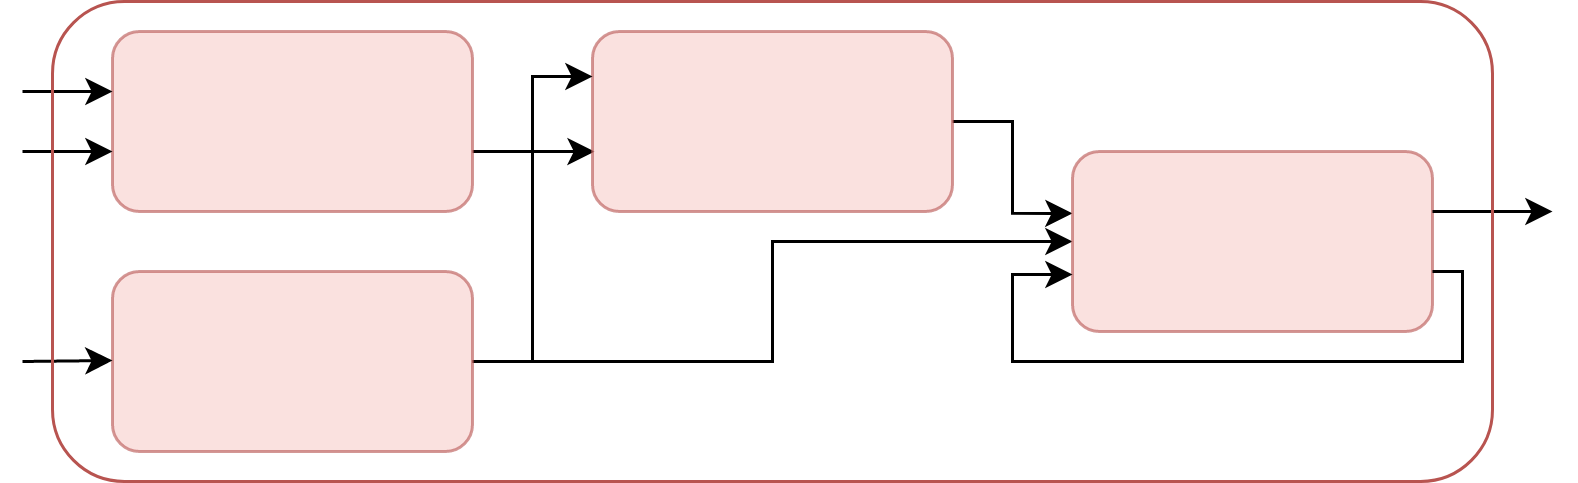
\includegraphics[scale=0.2]{graphics/lustre-nodes.png}
    \caption{A depiction of a dataflow program made up of nodes. The whole program accepts three inputs and computes
    one output. Notice that a node can depend on its output in the previous instant by feeding the output back as an input
    signal. This models a form of memory.}
    \label{graphics:dataflow}
\end{figure}

Drawing inspiration from this, french researchers in the 1980s did seminal work on \textit{synchronous} languages in the
form of the languages Lustre \cite{DBLP:conf/popl/CaspiPHP87}, Esterel \cite{DBLP:journals/scp/BerryG92},
and Signal \cite{DBLP:journals/scp/BenvenisteGJ91}. Lustre and Signal are dataflow languages, while Esterel
is an imperative language.

The two main concepts in Lustre are those of \textit{streams} and \textit{nodes}. A stream is an infinite sequence of values,
where a value need not be present at every instant. Consider the stream \code{X} that counts up at every instant, and
the stream \code{EVEN} that filters out the even numbers.

\begin{verbatim}
    instant 1,2,3,4,5,6,7,8,9,10,11,12,...

    X    = [1,2,3,4,5,6,7,8,9,10,...
    EVEN = [  2,  4,  6,  8,  10,...
\end{verbatim}

Whereas \code{X} is present at every instant, \code{EVEN} is only present at every other instant. New streams can be computed
from existing streams.

\begin{verbatim}
    X     = [1,2,3,4,5,...
    Y     = [6,2,3,4,9,...
    X + Y = [7,4,6,8,14,...
\end{verbatim}

The expression \code{X + Y} is only valid if \code{X} and \code{Y} are defined in the same instants. The expression
\code{X + Y} has no meaning if either \code{X} or \code{Y} doesn't have a value, and the program is rejected by the Lustre
compiler. It is common to refer to a stream as having a \textit{clock} that ticks at those instants where a value is
present. In the example with the streams \code{X} and \code{EVEN}, the clock of \code{X} ticks at a certain rate, and
the clock of \code{EVEN} ticks at half the rate of \code{X}.

As streams such as \code{X + Y} depend on other streams, \code{X + Y} \textit{reacts} when \code{X} and \code{Y} are
present. Reactions such as these are conceptually instantaneous, giving rise to the term \textit{synchronous} languages,
as inputs and outputs appear synchronised.

Esterel takes a different view of synchronicity. Instead of nodes in a dataflow graph reacting to input events, Esterel
declares nested threads that may react to broadcasted signals. Threads may suspend while waiting for a signal, and when
the signal is broadcasted in an instant, the thread reacts instantaneously. The signal does not persist until the next
instant. Esteral is an imperative language with common control-flow statements, such as loops and conditionals. While it
is not labeled as a dataflow language, the compiler will still construct a dataflow graph from the input and inspect it
to ensure that the program is deterministic.

These synchronous languages a compiled down to a single function that takes the inputs in the current instant and computes
the outputs. This function, which we refer to as the \textit{step}-function, is what conceptually finishes instantaneously.
Common to all these synchronous languages is that despite being able to create clocks and use them to specify
temporal behavior, a program is still ultimately governed by a global clock. Clocks can be derived from other clocks, such
as how the \code{EVEN} clock was derived from \code{X}, but regardless of which clock a node has, upon every tick of the
global clock, the step function is invoked. This is depicted in figure \ref{graphics:global-clock}.

Furthermore, while these synchronous languages were designed for specifying temporal properties, their sample-driven
nature makes them unable to specify concrete time values. A node can specify behavior in one instant, in relation to
other instants. There is not, however, a way to say e.g. \textit{wait for two seconds}. A node can have an input stream
that it assumes has a certain clock, but it is then up to the runtime system to supply the requested clock.

Stephen A. Edwards and John Hui \cite{DBLP:conf/fdl/EdwardsH20} recognized that giving meaning to every instant by invoking the
step function at every tick of a global clock can be
wasteful. In some application domains, such that that of \textit{Internet of Things}, a device may spend long periods doing nothing. During these periods, regardless of whether they are periodic or aperiodic, the program should not
have to react to any clock events. This lets the device the program executes on conserve power. This observation,
together with a desire to be able to specify concrete, precise temporal behavior natively, lead to the
\textit{Sparse Synchronous Model} (SSM).

In SSM, not all instants are assigned meaning, as shown in \ref{graphics:sparse-clock}. Temporal behavior such as
\textit{wait for two seconds} can be expressed natively, as computation is not driven by a base clock. Time is a
first-class citizen, and can be treated as any other value. As time is not expressed in terms of instants, but expressed
natively, it is possible to skip over instants. A SSM program is made up of processes, similar to Esterel. Threads may spawn
other threads and communicate to them via scheduled variables.

\begin{verbatim}
foo(&a)
  wait a
  a = a * 2

bar(&a)
  wait a
  a = a + 4

main()
  var a = 0
  after (1 second) a 1
  fork bar(a), foo(a)
\end{verbatim}

In the above example, the variable \code{a} is used to transmit signals. The \code{fork} statement will spawn concurrent
child processes \code{bar} and \code{foo}. The processes block until \code{a} receives an update, which it does after one second,
as scheduled by the \code{main} procedure before the children were forked. To ensure determinism, processes are ordered
by a priority that is derived from their parents' priority, and their syntactic order in a \code{fork} statement. The
above program will first give \code{a} the value \code{1} when one second has passed, after which \code{bar} wakes up and
adds \code{4} to it. Then \code{foo} wakes up and multiplies \code{a} with two, yielding a final value of \code{10} for \code{a}.

Another synchronous language that was developed at the same time as SSM is Lingua Franca (LF)
\cite{DBLP:journals/tecs/LohstrohMBL21}. LF uses the abstraction
of reactors instead of threads or nodes. Actors are used to model concurrent processes in languages such as Erlang. Actors
communicate by sending messages to each other but allow for non-determinism by not ordering messages.
The reactors in LF assign an ordering to every message, yielding a deterministic program.
A LF program, much like Lustre, declares a static dataflow graph, whereas SSM defines a dynamic dataflow graph that grows and shrinks as the
program is running.
Unique to LF is that it is a \textit{polyglot} language. The logic of each reactor can be given in many different
languages.

\begin{figure}
    \centering
    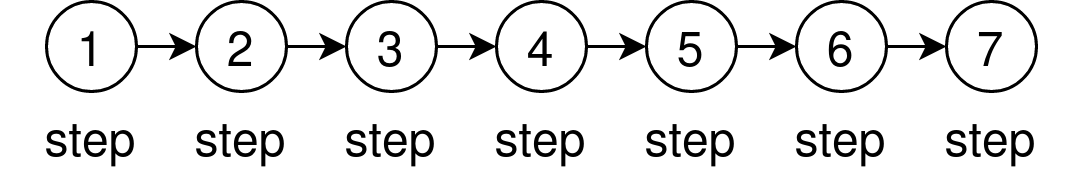
\includegraphics[scale=0.2]{graphics/clock-governed.png}
    \caption{Upon each tick of the global clock, the step function is invoked, and the whole program
    is evaluated for the instant denoted by the index of the tick.}
    \label{graphics:global-clock}
\end{figure}

\begin{figure}
    \centering
    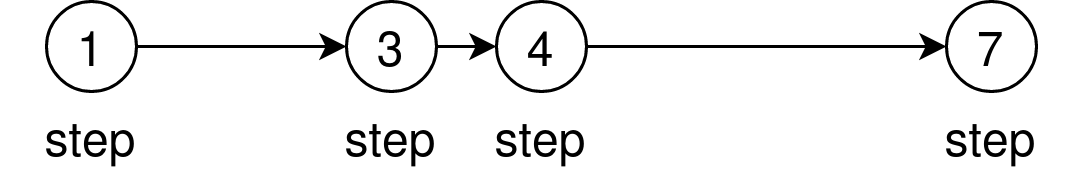
\includegraphics[scale=0.2]{graphics/sparse-clock.png}
    \caption{In contrast to the synchronous model, the sparse synchronous model allows the runtime system to
    not invoke the step function upon \textit{every} tick of the global clock.}
    \label{graphics:sparse-clock}
\end{figure}

\paragraph{Information-flow Control}

Information-flow control \cite{DBLP:series/natosec/HedinS12} (IFC) is a security mechanism that ensures that data propagates
through a program in such a way that some security policy is not violated. Values are labeled with a security level that is
tracked, and a value of one security level can not influence a value of a lower security level, as information
about the more secure value can leak to the value of a lower security level. The property that no data is leaked in this way is
called noninterference.

As a simple example, we describe a language with two security levels, public and secret. We assume that anyone can inspect
a program's public input and output. The pseudo-code below denotes security levels explicitly in the type signature
of the procedure.

\begin{verbatim}
    public int f(secret int x, public int y) {
        y = x;
        return y;
    }
\end{verbatim}

The above program is ill-formed, as the secret input is assigned to the public output before it is returned. This is an
explicit leakage of information. Implicit leakages are also possible, as in the program below.

\begin{verbatim}
    public bool f(secret bool x, public bool y) {
        if(x) {
            return y;
        } else {
            return (not y);
        }
    }
\end{verbatim}

By inspecting the output we can infer what the secret input was, even though we never directly assign the secret input
to the public variable \code{y}. Note that in both cases, the program would be accepted if we labeled the output as secret.

IFC policies can be enforced statically, dynamically, or through a combination of both. A static policy is checked before
a program is allowed to execute, whereas a dynamic policy is checked at runtime. If the policy is violated, execution
is aborted and an error is raised.

If a value could \textit{never} be downgraded to a lower security level, however, then it would be difficult to write any
meaningful program that uses different security levels. A principled way to release secrets is to explicitly declassify values,
giving them a lower security level.

\begin{verbatim}
secret string stored_pass;

public bool check_password(public string password) {
    secret outcome = compare(stored_pass, password);
    return declassify(outcome);
}
\end{verbatim}

The result of comparing the stored password against the candidate password must be secret, as we had to use the secret stored
password to do the comparison. Before the resulting boolean can be released as a public outcome, we must
\code{declassify} it.

Regardless of whether you use static IFC, dynamic IFC, or a hybrid variant of IFC, the threat model assumes that the
operating system and runtime system are trusted. In the presence of a compromised operating system, which we assume can
inspect any memory it desires, it does not matter what label a piece of data has. The operating system can inspect and
leak it. In this thesis, we investigate how we can strengthen this threat model by using TEEs to store the secret values.
Since the TEE does not need to trust the operating system, the secrets inside should remain safe even if the operating system
is compromised.

\paragraph{Trusted Execution Environments}

To protect data in use, every major hardware vendor is working on support for hardware-enforced trusted
execution environments (TEE). Intel is developing its Intel Software Guard Extensions (Intel SGX)\cite{intelsgx}, Arm is
developing Arm TrustZone\cite{armtz}, AMD is developing different variants such as AMD-SEV\cite{amdsev}, AMD-SME, and
AMD-SEV-SNP, to name just a few. A TEE allocates a contiguous region of memory that contains both secure code and data.
This region of memory is then protected by the hardware, where the protection mechanism varies between hardware vendors.
The purpose is that e.g. a compromised operating system can not read this memory.

Intel SGX refers to such protected memory regions as \textit{enclaves}, and protects them via encryption by the CPU. Code and
data are decrypted when they move into the CPU cache, and encrypted when it leaves the CPU cache. This constant encryption
and decryption add significant overhead. When untrusted code invokes a trusted method in an enclave, the time it takes
to just perform the function call is upwards of 35 times slower.

In contrast to Intel SGX, Arm TrustZone uses hardware isolation to separate the memory accessible by untrusted software and
trusted software. No encryption is needed, as untrusted memory can not access trusted memory. Performance seems to
be better than that of Intel SGX, but there are still overheads \cite{DBLP:conf/dais/AmacherS19} compared with using no TEE at all.

The programming model for TEEs requires the developer to partition their application into two components. One component
executes inside the TEE, while the untrusted component executes outside. The untrusted components drive the execution and may
perform remote procedure calls in the application inside the TEE, which in turn can call out of the enclave if it requires so.
If untrusted code tries to access trusted data, an error will be raised. This configuration is illustrated in
figure \ref{graphics:tee}.

\begin{figure}
    \centering
    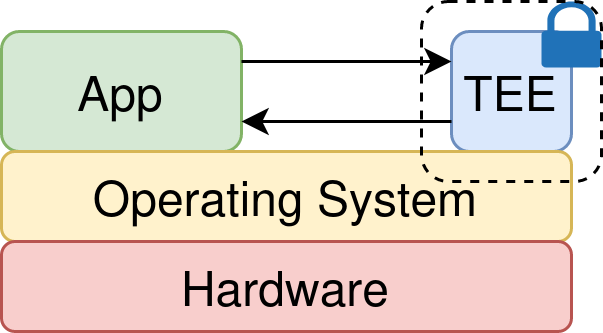
\includegraphics[scale=0.2]{graphics/tee.png}
    \caption{The diagram illustrates that an application using a hardware-enforced TEE to protect its secrets needs to
    be partitioned into two parts. The part outside of the TEE can perform remote procedure calls in the application
    executing inside the TEE. Arrows indicate remote procedure invocations.}
    \label{graphics:tee}
\end{figure}

While this sounds simple enough, it is in practice quite complicated. Aside from technical complexity
concerning the maintenance of toolchains, actual application development is not trivial. Managing two projects and an
interface between them takes some effort. The TEE application is much more restricted in what it can do as some
operations are inherently leaky. As an example, applications intended to run on Intel SGX need to be compiled with a
restricted version of the C standard library, where many ordinary functions are missing. This makes it difficult to port
legacy applications to run on Intel SGX, as these applications were written with the assumption that they can access the
whole standard library. To ease the porting of legacy applications to Intel SGX, projects such as Gramine have emerged
(previously called Graphene \cite{DBLP:conf/usenix/TsaiPV17}). Gramine is a library OS that reintroduces the missing
functionality from the restricted standard library, enabling any Linux binary to run unmodified.
